Listas de decisión es un algoritmo usado para resolver el problema de ambigüedad en el análisis del lenguaje natural con un porcentaje de acierto de incluso más del 90\% en las ambigüedades más complicadas. El algoritmo consiste en 7 pasos:\cite{DecisionLists}
\begin{enumerate}
    \item Identificar las ambigüedades que se quieren resolver:\\
    Por ejemplo los significados de palabras francesas que llevan acento. \cite{DecisionLists}\\ 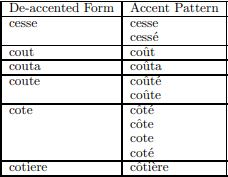
\includegraphics[]{img/listas/Listas_decision1.JPG}
    
    \item Recolectar los contextos para entrenar al algoritmo:\\
    Para esto es necesario construir oraciones que contengan las ambigüedades del punto anterior y que muestren diferentes contextos de uso. \cite{DecisionLists}\\
    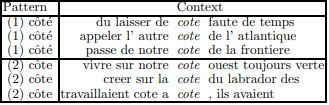
\includegraphics[]{img/listas/Listas_decision2.JPG}
    
    \item Medir como se distribuyen las palabras ambiguas:\\
    Para lograr esto se deben seguir las siguientes reglas:
    \begin{itemize}
        \item Por la palabra adyacente a la derecha de la ambigua será puntuada con $+1W$.
        \item Por la palabra adyacente a la izquierda de la ambigua, será puntuada con $-1W$.
        \item Por cada palabra a $k$ posiciones a la derecha de la ambigua será puntuada con $+kW$.
        \item Por cada palabra a $k$ posiciones a la izquierda de la ambigua será puntuada con $-kW$.
    \end{itemize}
    Entonces obtenemos una lista parecida a esta.\cite{DecisionLists}\\
    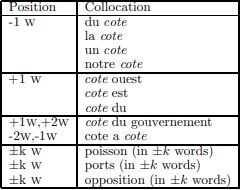
\includegraphics[]{img/listas/Listas_Decision3.JPG}
    
    \item Ordenar las tablas de forma descendente según la función de verosimilitud (log-likelihood\cite{log-likelihood}):\\
    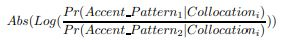
\includegraphics[]{img/listas/log-likelihood.JPG}\cite{DecisionLists}\\
    Dado que likelihood es una función de probabilidad necesitamos probabilidades que obtendremos de la data:\cite{DecisionLists}\\
    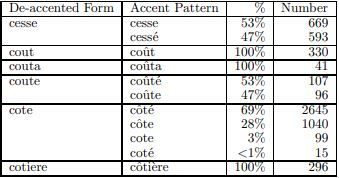
\includegraphics[]{img/listas/Listas_decision6.JPG}\\
    y terminaremos con una lista como esta:\cite{DecisionLists}\\
    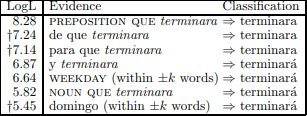
\includegraphics[]{img/listas/Listas_decision4.JPG}\\(notese que es de otro ejemplo)
    
    \item Opcionalmente podar e interpolar las listas
    \item Entrenar las listas para ambigüedades mas generales:\\
    Esto es cuando la palabra que causa la ambigüedad puede ser incluida en una clase o conjunto de palabras con usos similares.
    \item Usar las listas:\\
    Mientras se recorre el texto se revisa si a alguna palabra que se va leyendo le pertenece alguna lista de decisión, osea si se considera ambigua, ya sea de la misma palabra o de su clase, si es que pertenece a una clase. Si no se considera ambigua no pasa nada pero si sí, se recorre su lista hasta encontrar el mayor ranking que coincida con el contexto de la palabra ambigua.
\end{enumerate}

Análisis de la complejidad:
\begin{enumerate}
    \item Espacio:\\
    Supongamos que queremos analizar $n$ ambigüedades de las cuales el máximo de significados que alguna pueda tener es $k$ y queremos entrenar a la lista para reconocer estos significados en un máximo de $c$ contextos. Entonces tendríamos $n$ listas de tamaño $O(kc)$. Lo cual nos deja con una complejidad de $O(nkc)$ space.
    \item Tiempo:
    \begin{itemize}
        \item Para armar las listas:\\
        Obviando el paso opcional 5, para calcular la tabla solo se efectúan 2 operaciones: la medición de como se distribuyen las palabras ambiguas en el contexto y el ordenamiento de las listas según el resultado de la función log-likelihood.\\Para realizar la primera operación no se especifica ningún algoritmo así que supondremos que existe uno de complejidad $O(m)$ para puntuar las palabras de un contexto con un número máximo de $m$ palabras y sabiendo que la lista tiene un tamaño total de $n$ contextos podemos decir que la complejidad resultante de este paso es de $O(nm)$ time.\\Para la segunda operación sabemos que para una variable discreta, a diferencia de su forma para variables continuas, log-likelihood es una función matemática que no requiere del uso de métodos numéricos así que tiene una complejidad $\Theta(1)$ y para aplicarla a $n$ elementos de la lista se necesita $\Theta(n)$ time. Y una ves calculados estos valores deberá ser ordenada, para lo cual cualquier algoritmo de ordenamiento eficiente servira asi que supondremos uno de complejidad $O(nLog(n))$ time. Entonces $\Theta(n)+O(nLog(n))=O(nLog(n))$ time.
        \item Para usar las listas:\\
        Siguiendo las instrucciones indicadas en el paso 7 podemos intuir que se realiza un recorrido lineal a través de la lista lo cual nos daría un peor escenario de complejidad $O(n)$ time donde $n$ son las filas de la lista. Sin embargo, debido a que los elementos están ordenados de forma descendente en la probabilidad de ser el significado real obtenemos un escenario promedio de complejidad $O(1)$ time. Y con $p$ palabras ambiguas en la conseguimos la resolución de la ambigüedad en una cota inferior de $\Omega(p)$ y en una cota superior de $O(pn)$.
    \end{itemize}
\end{enumerate}